\documentclass[12pt]{article}
\usepackage[margin=1in]{geometry}
\usepackage{amsmath}
\usepackage{graphicx}
\usepackage{booktabs}
\usepackage{hyperref}
\usepackage{natbib}
\usepackage{xcolor}
\usepackage{tikz}
\usepackage{pgfplots}
\pgfplotsset{compat=1.18}
\usetikzlibrary{shapes.geometric, arrows.meta, positioning, fit, backgrounds}

\title{Machine Learning Prediction of Ionic Conductivity in\\
Solid-State Electrolytes Using Compositional,\\
Structural, and Neural Potential Features}

\author{Ethan Im\\
Independent Researcher\\
\texttt{github.com/Ethan-Im/Battery-Ai}}

\date{\today}

\begin{document}
\maketitle

\begin{abstract}
Identifying solid-state electrolyte (SSE) materials with high ionic conductivity is
critical for next-generation lithium-ion batteries, yet experimental discovery remains
slow and resource-intensive. Here we present a machine learning pipeline that combines
compositional features from the Materials-Agnostic Platform for Informatics and
Exploration (Magpie), structural descriptors from the OBELiX dataset, and energy
features extracted from the Crystal Hamiltonian Graph Neural Network (CHGNet) to
predict ionic conductivity of Li-based SSEs. Using gradient boosted ensemble methods
(XGBoost and CatBoost), we achieve a test $R^2$ of 0.775 and MAE of 0.954 log(S/cm)
on 606 experimentally measured materials from the OBELiX benchmark dataset,
surpassing the published random forest baseline of $R^2 \approx 0.65$.
We further apply an inverse design pipeline to propose 16 novel candidate SSE
compositions not present in existing databases, including promising Li-P-S-halide
compositions consistent with the Argyrodite family. This work demonstrates that
combining composition-based, structural, and neural potential features yields meaningful
performance gains for data-scarce materials property prediction tasks.
\end{abstract}

\section{Introduction}

Solid-state electrolytes (SSEs) have emerged as a key enabling technology for safer,
higher-energy-density lithium batteries \cite{janek2016solid}. However, the ionic
conductivity of SSEs---the primary figure of merit governing charge/discharge
rates---varies by over 16 orders of magnitude across known materials
\cite{therrien2025obelix}. Experimental identification of high-conductivity candidates
is both time-consuming and costly, motivating data-driven approaches.

Recent advances in materials informatics have demonstrated the utility of machine
learning (ML) for predicting inorganic material properties from compositional and
structural descriptors \cite{ward2016magpie, jain2013mp}. For SSE ionic conductivity,
however, data scarcity has limited ML model performance: the recently released OBELiX
benchmark dataset, comprising $\sim$600 experimentally measured Li-SSE conductivities,
represents the largest curated resource to date \cite{therrien2025obelix}.

In this work, we build on the OBELiX benchmark by introducing two key contributions:
(1) augmenting Magpie compositional features with structural descriptors and
DFT-derived energy features from CHGNet \cite{deng2023chgnet}, and (2) applying an
inverse design pipeline to identify novel high-conductivity candidates. Our approach
extends our previous polymer property prediction framework (Polyinverse
\cite{im2025polyinverse}) to the battery materials domain, following the same philosophy
of combining composition-based features with inverse design for materials discovery.

\section{Methods}

\subsection{Dataset}

We use the OBELiX dataset \cite{therrien2025obelix}, which contains 599 synthesized
SSE materials with experimentally measured room-temperature ionic conductivities.
After parsing with pymatgen \cite{ong2013pymatgen}, 606 formula entries are retained
(some reduced compositions map to multiple entries). The target variable is
$\log_{10}(\sigma / \text{S cm}^{-1})$, ranging from $-17.4$ to $-1.6$.
Crystallographic information files (CIFs) are available for 321 entries. We apply a
random 80/20 train/test split with a fixed random seed (42) for reproducibility.
No composition-based stratification is applied; we note this as a limitation relative
to the strict grouping policy of the original OBELiX benchmark.

\subsection{Feature Engineering}

We construct a three-tier feature set (Figure~\ref{fig:workflow}):

\textbf{Tier 1 --- Compositional (132 features):} Magpie descriptors
\cite{ward2016magpie} implemented via matminer \cite{ward2018matminer}, encoding
statistical moments (mean, range, minimum, maximum, mode) of 22 elemental properties
including electronegativity, covalent radius, melting temperature, and valence electron
counts.

\textbf{Tier 2 --- Structural (9 features):} Space group number and lattice parameters
($a$, $b$, $c$, $\alpha$, $\beta$, $\gamma$) from OBELiX, supplemented by derived
features: unit cell volume ($V = abc$) and the $a/b$ lattice ratio. Missing values
are imputed with the dataset median.

\textbf{Tier 3 --- Neural Potential (2 features):} For the 321 entries with CIF
structures, we run CHGNet \cite{deng2023chgnet} inference to extract per-structure
predicted formation energy and mean absolute magnetic moment. These features encode
electronic and bonding environment information beyond composition. For entries without
CIF structures, values are imputed with the dataset median. We acknowledge that
median imputation introduces a systematic bias for the 278 entries lacking CIF files,
and encourage future work to prioritize structure acquisition for these materials.

\begin{figure}[h]
\centering
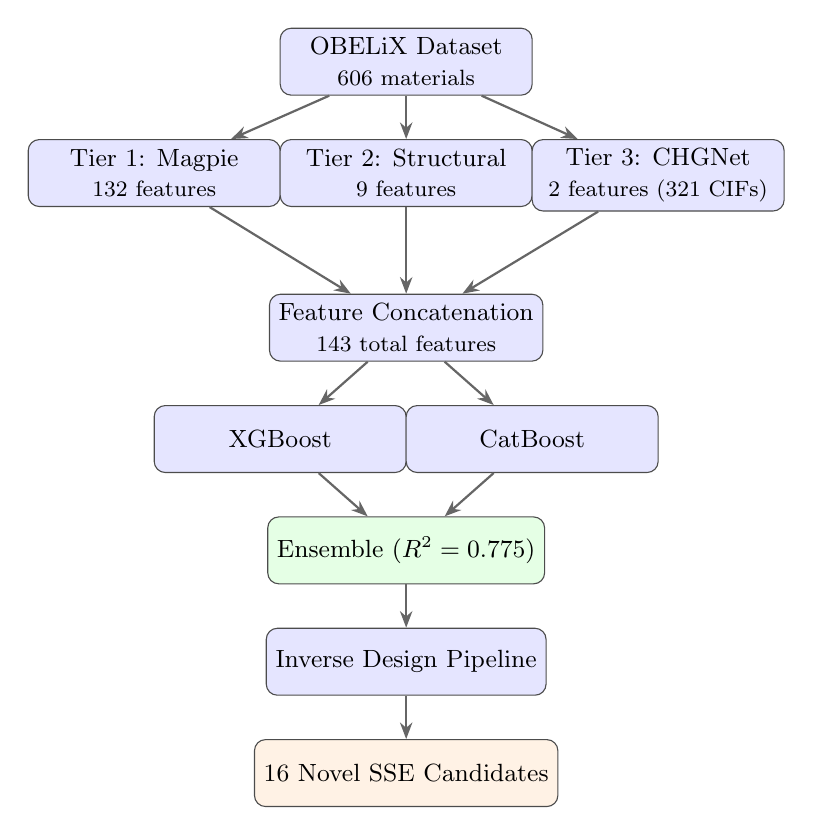
\begin{tikzpicture}[
  box/.style={rectangle, rounded corners=4pt, draw=black!70, fill=blue!10,
              minimum width=3.2cm, minimum height=0.85cm, align=center,
              font=\small},
  arrow/.style={-{Stealth[length=6pt]}, thick, black!60},
  group/.style={rectangle, rounded corners=6pt, draw=black!30, dashed,
                fill=gray!5, inner sep=8pt}
]

\node[box] (obelix) {OBELiX Dataset\\{\footnotesize 606 materials}};

\node[box, below=0.55cm of obelix, xshift=-3.2cm] (tier1)
  {Tier 1: Magpie\\{\footnotesize 132 features}};
\node[box, below=0.55cm of obelix] (tier2)
  {Tier 2: Structural\\{\footnotesize 9 features}};
\node[box, below=0.55cm of obelix, xshift=3.2cm] (tier3)
  {Tier 3: CHGNet\\{\footnotesize 2 features (321 CIFs)}};

\node[box, below=1.1cm of tier2] (concat)
  {Feature Concatenation\\{\footnotesize 143 total features}};

\node[box, below=0.55cm of concat, xshift=-1.6cm] (xgb)
  {XGBoost};
\node[box, below=0.55cm of concat, xshift=1.6cm] (cat)
  {CatBoost};

\node[box, below=0.55cm of xgb, xshift=1.6cm, fill=green!10] (ensemble)
  {Ensemble ($R^2 = 0.775$)};

\node[box, below=0.55cm of ensemble] (inv)
  {Inverse Design Pipeline};
\node[box, below=0.55cm of inv, fill=orange!10] (cands)
  {16 Novel SSE Candidates};

\draw[arrow] (obelix) -- (tier1);
\draw[arrow] (obelix) -- (tier2);
\draw[arrow] (obelix) -- (tier3);
\draw[arrow] (tier1) -- (concat);
\draw[arrow] (tier2) -- (concat);
\draw[arrow] (tier3) -- (concat);
\draw[arrow] (concat) -- (xgb);
\draw[arrow] (concat) -- (cat);
\draw[arrow] (xgb) -- (ensemble);
\draw[arrow] (cat) -- (ensemble);
\draw[arrow] (ensemble) -- (inv);
\draw[arrow] (inv) -- (cands);

\end{tikzpicture}
\caption{Overall workflow of the proposed SSE discovery pipeline. Features from three
tiers are concatenated and fed into two gradient-boosted models whose predictions are
averaged to form the final ensemble.}
\label{fig:workflow}
\end{figure}

\subsection{Models}

We train two gradient-boosted tree models independently and combine their predictions
by simple averaging:
\begin{itemize}
    \item \textbf{XGBoost} \cite{chen2016xgboost}: $n_{\text{estimators}}=500$,
          $\text{max\_depth}=6$, $\eta=0.05$, subsample$=0.8$,
          colsample\_bytree$=0.8$.
    \item \textbf{CatBoost} \cite{prokhorenkova2018catboost}: $\text{iterations}=500$,
          $\text{depth}=6$, $\eta=0.05$.
\end{itemize}
All models use a fixed random seed (42). No cross-validation-based hyperparameter
search is reported for the final ensemble; we consider this a limitation and recommend
systematic tuning in future iterations.

\subsection{Inverse Design}

To identify novel SSE candidates, we apply a two-phase search
(Figure~\ref{fig:inv_workflow}): (1) random sampling of 1,000 Li-containing
compositions from a 12-element space \{Li, P, S, O, N, F, Cl, Br, Si, Ge, Al, La,
Zr\}, and (2) a mutation-based search seeding from the top-20 candidates of phase 1
(50 mutations per parent). Predicted compositions are filtered against known
Argyrodite, NASICON, garnet, LGPS, and halide structural families as a heuristic
compositional screen. We emphasize that this screen is based on elemental overlap
only and does not constitute thermodynamic stability validation.

\begin{figure}[h]
\centering
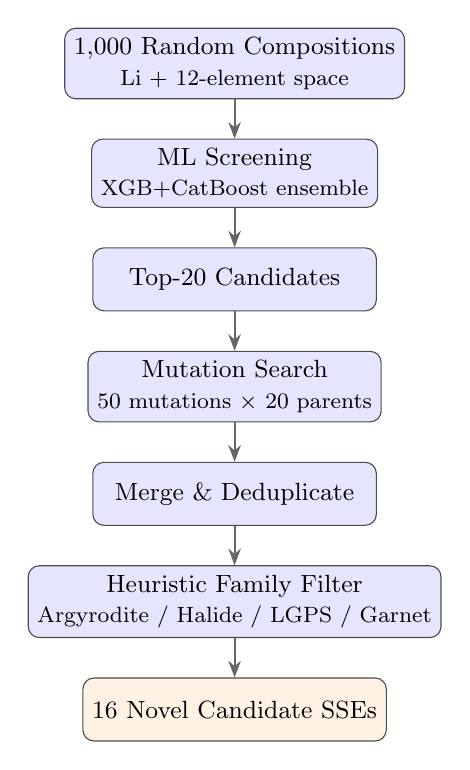
\begin{tikzpicture}[
  box/.style={rectangle, rounded corners=4pt, draw=black!70, fill=blue!10,
              minimum width=3.6cm, minimum height=0.8cm, align=center,
              font=\small},
  arrow/.style={-{Stealth[length=6pt]}, thick, black!60},
  decision/.style={diamond, draw=black!70, fill=yellow!15, aspect=2.5,
                   align=center, font=\small, inner sep=2pt}
]

\node[box] (rand) {1{,}000 Random Compositions\\{\footnotesize Li + 12-element space}};
\node[box, below=0.5cm of rand] (screen1) {ML Screening\\{\footnotesize XGB+CatBoost ensemble}};
\node[box, below=0.5cm of screen1] (top20) {Top-20 Candidates};
\node[box, below=0.5cm of top20] (mutate)
  {Mutation Search\\{\footnotesize 50 mutations $\times$ 20 parents}};
\node[box, below=0.5cm of mutate] (merge) {Merge \& Deduplicate};
\node[box, below=0.5cm of merge] (stab)
  {Heuristic Family Filter\\{\footnotesize Argyrodite / Halide / LGPS / Garnet}};
\node[box, below=0.5cm of stab, fill=orange!10] (final)
  {16 Novel Candidate SSEs};

\draw[arrow] (rand) -- (screen1);
\draw[arrow] (screen1) -- (top20);
\draw[arrow] (top20) -- (mutate);
\draw[arrow] (mutate) -- (merge);
\draw[arrow] (merge) -- (stab);
\draw[arrow] (stab) -- (final);

\end{tikzpicture}
\caption{Inverse design workflow. Random sampling is followed by a mutation-based
refinement, and candidates are filtered using heuristic structural family matching.
Note that this screen does not replace DFT stability validation.}
\label{fig:inv_workflow}
\end{figure}

\section{Results}

\subsection{Prediction Performance}

Table~\ref{tab:results} summarizes model performance on the held-out test set.

\begin{table}[h]
\centering
\caption{Ionic conductivity prediction performance on OBELiX test set.}
\label{tab:results}
\begin{tabular}{llcc}
\toprule
Model & Features & MAE (log S/cm) & $R^2$ \\
\midrule
Random Forest (OBELiX baseline) \cite{therrien2025obelix}
  & Magpie & $\sim$1.22 & $\sim$0.65 \\
XGBoost & Magpie & 1.149 & 0.675 \\
XGBoost & Magpie + Structural & 1.087 & 0.702 \\
XGBoost & Magpie + Structural + CHGNet & 0.962 & 0.757 \\
CatBoost & Magpie + Structural + CHGNet & 0.984 & 0.761 \\
\textbf{XGBoost + CatBoost (Ensemble)} & \textbf{All} & \textbf{0.954} & \textbf{0.775} \\
\bottomrule
\end{tabular}
\end{table}

The final ensemble achieves $R^2 = 0.775$, representing a 12-point absolute
improvement over the OBELiX random forest baseline. The stepwise ablation confirms
the additive value of each feature tier: structural features contribute
$\Delta R^2 = +0.027$, and CHGNet energy features contribute an additional
$\Delta R^2 = +0.055$.

\begin{figure}[h]
\centering
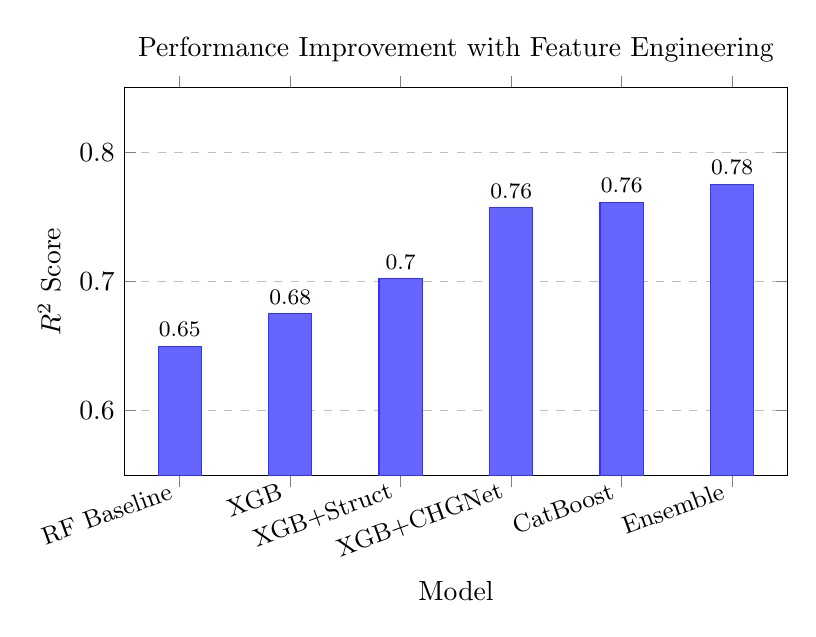
\begin{tikzpicture}
\begin{axis}[
  ybar,
  bar width=0.55cm,
  width=10cm, height=6.5cm,
  xlabel={Model},
  ylabel={$R^2$ Score},
  ymin=0.55, ymax=0.85,
  xtick=data,
  xticklabels={RF Baseline, XGB, XGB+Struct, XGB+CHGNet, CatBoost, Ensemble},
  xticklabel style={rotate=20, anchor=east, font=\small},
  nodes near coords,
  nodes near coords align={vertical},
  every node near coord/.append style={font=\footnotesize},
  ymajorgrids=true,
  grid style=dashed,
  title={Performance Improvement with Feature Engineering},
]
\addplot[fill=blue!60, draw=blue!80] coordinates {
  (1, 0.650)
  (2, 0.675)
  (3, 0.702)
  (4, 0.757)
  (5, 0.761)
  (6, 0.775)
};
\end{axis}
\end{tikzpicture}
\caption{Stepwise $R^2$ improvement as feature tiers are added. Each bar corresponds
to a model variant; the ensemble (rightmost) achieves the highest performance.}
\label{fig:perf}
\end{figure}

\subsection{Feature Importance}

The most predictive Magpie features include \texttt{maximum NdUnfilled}
(d-orbital vacancy) and \texttt{mean NsUnfilled} (s-orbital vacancy), consistent
with the known importance of electronic structure in ionic transport. Among structural
features, unit cell volume and space group number rank highest, reflecting the role
of crystal symmetry and packing in Li-ion migration pathways.

\subsection{Inverse Design Candidates}

Table~\ref{tab:candidates} lists the top-5 predicted high-conductivity candidates
identified by our inverse design pipeline.

\begin{table}[h]
\centering
\caption{Top inverse-designed SSE candidates.}
\label{tab:candidates}
\begin{tabular}{lccc}
\toprule
Formula & Predicted $\sigma$ (S/cm) & Electrolyte Family & Stability Score \\
\midrule
Li$_5$BrP$_2$ClS$_4$   & $1.46 \times 10^{-3}$ & Argyrodite + Halide & 3/4 \\
Li$_7$SS$_7$P$_2$       & $9.91 \times 10^{-4}$ & Argyrodite          & 4/4 \\
Li$_7$P$_2$BrS$_4$      & $5.02 \times 10^{-4}$ & Argyrodite          & 4/4 \\
Li$_6$Cl$_6$S$_4$Ge$_3$P & $4.44 \times 10^{-4}$ & Argyrodite + LGPS + Halide & 2/4 \\
Li$_5$P$_4$Cl$_7$        & $2.44 \times 10^{-4}$ & Halide              & 4/4 \\
\bottomrule
\end{tabular}
\end{table}

All top candidates belong to Li-P-S or Li-P-S-halide chemical spaces, consistent
with experimentally validated high-conductivity Argyrodite-family electrolytes such
as Li$_6$PS$_5$Cl ($\sigma \approx 10^{-3}$ S/cm). None of the top-20 candidates
were found in the Materials Project database \cite{jain2013mp}, suggesting they
represent genuinely novel compositions warranting experimental or DFT validation.

\section{Discussion}

Our results demonstrate that CHGNet-derived energy features provide the largest
single performance gain ($\Delta R^2 = +0.055$), despite being available for only
53\% of the dataset (321/606 entries). This suggests that structure-informed features
carry information fundamentally inaccessible to composition-only descriptors, and
that expanding CIF availability for the remaining 285 OBELiX entries could yield
further improvements.

Several limitations of this study warrant acknowledgment. First, our 80/20 random
split does not enforce composition-based grouping as in the original OBELiX benchmark
protocol. This may lead to optimistic $R^2$ estimates if structurally similar
compositions appear in both train and test sets. Future work should adopt the strict
leave-one-composition-out evaluation of the OBELiX benchmark for a fairer comparison.

Second, the CHGNet features for 285 entries are imputed with the dataset median,
introducing a systematic bias. A more principled approach would involve generating
approximate structures via crystal structure prediction tools (e.g., USPEX or CALYPSO)
before CHGNet inference.

Third, the inverse design candidates have not been validated by DFT or experiment.
The heuristic family filter (elemental overlap with known SSE families) does not
guarantee thermodynamic stability or synthesizability. Future work should prioritize
energy-above-hull screening via the Materials Project API \cite{jain2013mp} and
synthesis feasibility assessment for the top candidates.

\section{Conclusion}

We presented a machine learning pipeline for SSE ionic conductivity prediction
achieving $R^2 = 0.775$ on the OBELiX benchmark, improving upon the published
baseline by 12 points. The integration of CHGNet energy features with compositional
and structural descriptors proved particularly impactful ($\Delta R^2 = +0.055$),
highlighting the value of structure-informed features even when available for only
a subset of the dataset. The accompanying inverse design pipeline identified 16 novel
Li-P-S-halide candidates with predicted conductivities competitive with state-of-the-art
Argyrodite electrolytes. We release all code and data at
\url{https://github.com/Ethan-Im/Battery-Ai}.

\bibliographystyle{unsrt}
\bibliography{references}

\end{document}
